\chapter{Reliability of the SPI protocol and FPGA implementation}
\label{sec:spi_rel_test}
This experiment has the purpose of testing how reliable the implemented SPI hardware and protocol is. 

\section{Range}	% (Which system part is tested?)
The SPI interface will be tested as a stand alone unit-test, so no other hardware has access to read or write the shared memory as this could effect the test results. The test will be done by generating 32 random bytes, writing these to the memory on the FPGA. Afterwards the 32 bytes will be read from the FPGA and compared with the bytes send. To test the performance in noisy environments, different cables length are used. It is a goal to find out how long distance data can be transferred without errors starting to occur, and to determine how reliable FPGA hardware is.

%The position will shift between two different positions and the positions will be recorded when the controller believes the position is reached. When controller stops the position are marked, and the other position is set to the controller and this position are now marked etc. This is repeated ten times.

\section{Test Setup}
The test setup is done by isolating the SPI hardware and memory on the FPGA. An Arduino\footnote{\url{http://arduino.cc}} is connected as master to the FPGA SPI interface, and by a serial port to a computer. The Arduino has been programmed to pass serial data to the SPI hardware and SPI data to the serial port. The SPI will in this test run at a speed of 4MHz. A C\#.net application has been written to generate random bytes, write them to the memory, read them back, compare and log the results. This allows easy testing of the hardware with different configurations. The C\# software is considered a black box testing tool in this project. It is not be described in greater details, but it is included on the CD. Figure \ref{fig:spi_testapplication} shows a picture of the testing software in progress. A big textbox shows the test log, and a small textbox on the right outputs the CSV data with the test results.

For every cable length in the test, the read/write process is done 100 times to give a good average on the results. The test is started with a long cable, which are then shorted between every test to give an idea about a what length the errors starts to occur. The test with short cables will show if the FPGA hardware is able to communicate without error.

Nothing will be done to avoid electric noise in the test. But all test will be made in the same environment to make the results comparable.

\begin{figure}[htb] 
	\centering
	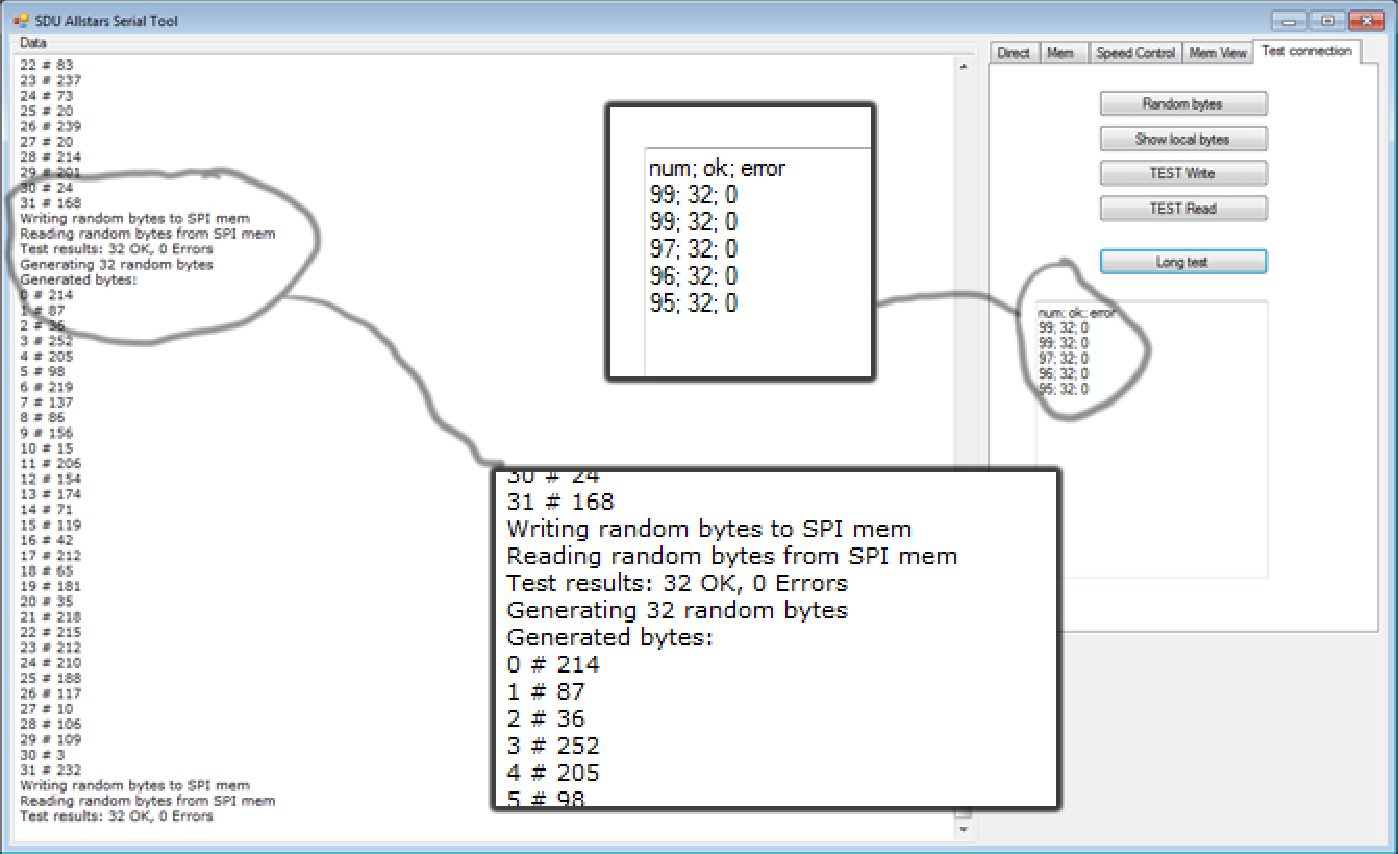
\includegraphics[width=\textwidth,trim=0 0 0 0]{graphics/spi_testapplication.pdf} %trim=l b r t (can cut off from every side)
	\caption{Tool for testing the reliability of the FPGA SPI hardware.}
	\label{fig:spi_testapplication}			% figure labels are of the form \label{fig:*}
\end{figure}


\section{Result}
The test turned out quite unexpected. It was expected that at some length, a small amount of errors would start to occur and then slowly rise while the cable length was increased until no data could be transferred correctly. The test shows that data can be transferred successfully with cables up to 25cm, and then errors starts to occur, but at a length of 75cm the error does not increase dramatic by increasing the length of the cable.

\begin{table}[htb]								%[htb] means here, top or bottom (where latex tries to place the float on the page)
	\centering
	\begin{tabular}{cccc}					% | is a vertical line ; c means center, l left and r right
	Cable length & Correct read/writes [Bytes] & Bad read/writes [Bytes] & Error pct. \\			% the &-sign seperates columns
	\midrule													%horizontal line
	0,1m & 3200 & 0 & 0\%  \\
	0,25 & 3200 & 0 & 0\% \\
	0,5 & 700 & 500 & 15,6\% \\
	0,75m & 675 & 2525 & 78,9\% \\
	1,0m & 678 & 2522 & 78,8\% \\
	1,5m & 645 & 2555 & 79,8\% \\
	2,0m & 654 & 2546 & 79,6\% \\
	2,5m & 356 & 2844 & 88,8\%
	\end{tabular}
	\caption{Results from SPI test.}				% The caption (billedtekst!). All floats should have a caption
	\label{tab:spi_test_results}			% reference ID. Tables are of the format \label{tab:*}
\end{table}

The data from the test were logged, but no further analyses will be needed in this test, it is though included on the CD for further studies.

A thing to note about the test, is that nothing was done to actively disturb the transmission. If a disturbing element were present the transmission would probably experience a higher rate of errors. If the transmission was to be used in a noisy environment, a protocol including error detection or correction would need to be implemented instead.


\section{Conclusion}
The test concludes that data successfully can be sent and received correctly at a speed of 4MHz at distances up to 25cm. At distances below 25cm the communication has 0\% error transmission, which shows that the hardware implemented on the FPGA can work without errors.